\documentclass[a4paper,12pt]{article}
\usepackage{graphicx, float, fancyheadings, a4wide, makeidx, verbatim,avant,helvet}
\usepackage{}
\pagestyle{fancyplain}
\setlength{\parindent}{0pt}
\setlength{\parskip}{6pt}

\newcommand{\param}[1] {\textless{}#1\textgreater{}}

\title{\sf{Datasheet for Temperature Sensors}}
\lfoot{\tiny{\copyright L.P.Klyne}}

\author{Andy Harris}

\makeindex

\begin{document}

\maketitle

\begin{figure}[H]
\centering

\includegraphics[width=0.4\textwidth]{Images/WebBrickSystems.png}
\end{figure}

\begin{figure}[H]
\centering

\includegraphics[width=0.3\textwidth]{Images/wb_logo.jpg}
\end{figure}


\begin{description}
\item[Feb 2007 Document Version 1.02]
\end{description}

\begin{description}
\item[http:\\www.WebbrickSystems.com] for company information
\item[http:\\www.webbrick.co.uk] for webbrick information
\end{description}

\pagebreak

\section{Temperature Sensors}
\index{Temperature Sensors}

\begin{figure}[H]
\centering
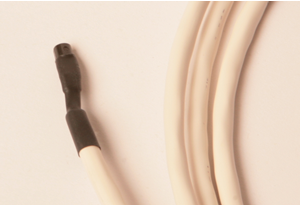
\includegraphics[width=0.4\textwidth]{Images/TempSensorPic.png}
\end{figure}

\subsection{WebBricks and Temperature Sensors}

We supply and recommend Dallas DS18B20 temperature sensors.  These are connected to the 1 Wire bus on the WebBrick
within the following limits:

	\begin{itemize}
	  
	  \item{Cable:} Cat 5E cable is recommended for temperature sensor connections.  Webbrick Systems supply
	  		temperature sensors with 2M Cat 5E pre-attached.
	  		
	  \item{Bus Length:}  We recommend a maximum bus length of 90M for a single sensor and 50M for multiple sensors.
	  			Maximum spur length 2M.
	  			
	  \item{Unused cores:} We recommend that unused cores are connected to ground.  In particular the brown core
	  			should be connected to ground.
	  			
	  \item{Sensor Accuracy:} Is within 0.5 Deg C.
	  
	  \item{Sensor Resolution:} Is 0.125 Deg C, although this is less than the accuracy of the temperature sensor
	  				it is very useful for determination of whether a temperature is rising or falling
	  
	\end{itemize}


\subsection{Connections}

The following connections should be made:

\begin{figure}[H]
\centering
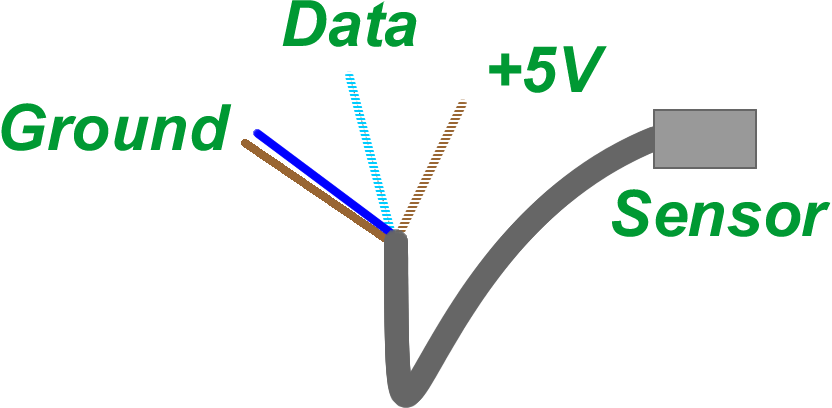
\includegraphics[width=0.6\textwidth]{Images/TempSensor.png}
\end{figure}

	\begin{itemize}
	  
	  \item{Brown-White:} +5V
	  		
	  \item{Blue-White:} Data 

	  \item{Blue:} Ground 

	  \item{Brown:} Ground, this core is not connected to the temperature sensor,
	  		grounding this core satisfies the EMC conditions of CE marking.
	  			
	\end{itemize}


Note that multiple temperature sensors are connected in parallel.


\end{document}
